\subsection{Limite des bases de données relationnelles :}
Les bases de données existent maintenant depuis environ 56 ans et le modèle relationnel depuis environ 46 ans, pendant plusieurs décennies, ce modèle bien très puissant, représentait la solution parfaite pour les différents acteurs dans le domaine de gestion des données, néanmoins ces architectures ont atteints leurs limites pour certains services ou sites manipulant de grandes masses de données, tels que Google, Facebook, etc. En effet ce genre de sites possède plusieurs millions voire des milliards d’entrées dans leurs bases de données et tout autant de visites journalières, en conséquence les données sont distribuées sur plusieurs machines, de plus pour des raisons de fiabilité ces bases de données sont dupliquées pour que le service ne soit pas interrompu en cas de panne.

Malheureusement le modèle relationnel présente quelques problèmes liés à ce passage à l’échelle tel que :

\subsubsection{1. Problème lié à l’application des propriétés ACID en milieu distribué :}
Une base de données relationnelle est construite en respectant les propriétés ACID (Atomicité, Cohérence, Isolation, Durabilité), ses propriétés bien que nécessaires à la logique du relationnel nuisent fortement aux performances et en particulier la propriété de cohérence.

En effet, la cohérence est très difficile à mettre en place dans le cadre de plusieurs serveurs (environnement distribué), car pour que celle-ci soit respectée tous les serveurs doivent être des miroirs les uns des autres, de ce fait deux problèmes apparaissent :
\begin{itemize}[label=\textbullet]
\item Le coût en stockage est énorme car chaque donnée est présente sur chaque serveur.
\item Le coût d’insertion/modification/suppression est très grand, car on ne peut valider une transaction que si on est certain qu’elle a été effectuée sur tous les serveurs et le système fait patienter l’utilisateur durant ce temps.
\end{itemize}

\begin{figure}[h]
	\centering
    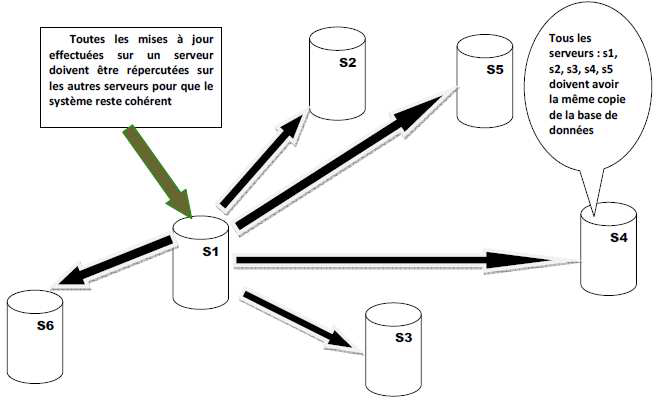
\includegraphics[scale=0.5]{img/4.0.2}
    \caption{Problème lié aux propriétés ACID en milieu distribué}
\end{figure}

\subsubsection{2. Pas de schéma de base de données hiérarchique :  }
Contrairement aux bases de données orientées objet, les bases de données relationnelles n'offrent pas la possibilité d'implémenter des schémas de base de données avec des classes hiérarchiquement structurées. Des concepts tels que les entités subordonnées qui héritent de propriétés d'entités supérieures ne peuvent pas être implémentés avec elles. Par exemple, on ne peut pas créer de sous-tuples avec eux. Tous les tuples d'une base de données relationnelle se trouvent au même niveau hiérarchique.

\subsubsection{3. Problème de requête non optimale dû à l’utilisation des jointures :}
Imaginons une table contenant toutes les personnes ayant un compte sur Facebook, soit 1.55 milliards d’utilisateurs actifs par mois les données dans une base de données relationnelle classique sont stockées par lignes, ainsi si on effectue une requête pour extraire tous les amis d’un utilisateur donné, il faudra effectuer la jointure entre la table des usagers et celle des amities (chaque usagr ayant au moins un ami) puis parcourir le produit cartésien de ces deux tables. De ce fait, on perd énormément en performances en raison du temps consommé pour stocker et parcourir une telle quantité de données.

\subsubsection{4. Problème lié à la gestion des objets hétérogènes: }

« Le stockage distribué n’est pas la seule contrainte qui pèse à ce jour sur les systèmes relationnels» disait Carl STROZZI. Au fur et à mesure du temps, les structures de données manipulées par les systèmes sont devenues de plus en plus complexes en contrepartie les moteurs de stockage évoluant peu. Le principal point faible des modèles relationnels est l’absence de gestion d’objets hétérogènes ainsi que le besoin de déclarer au préalable l’ensemble des champs représentant un objet.

D’autre part le modèle relationnel est fondé sur un modèle mathématique solide s’appuyant sur des concepts simples qui font sa force en même temps que sa faiblesse.

Nous expliquerons quelques limites :

\begin{enumerate}
\item \textbf{Surcharge sémantique :} Le modèle relationnel s’appuie sur un seul concept (la relation) pour modéliser à la fois les entités et les associations entre ces entités. Il existe donc un décalage entre la réalité et sa représentation abstraite.
\item \textbf{Types de données :} Ces modèles sont limités à des types simples (entiers, réels, chaînes de caractères), les seuls types étendus se limitant à l’expression de dates ou de données financières, ainsi que des conteneurs binaires de grande dimension (BLOB, pour Binary Large OBjects) qui permettent de stocker des images ainsi que des fichiers audio ou vidéos. Ces BLOBs ne sont toutefois pas suffisants pour représenter des données complexes (pas de structure), les mécanismes de contrôle BD sont inexistants, et le langage de requêtes (SQL) ne possède pas les opérateurs correspondant aux objets stockés dans ces BLOBs.
\end{enumerate}

\subsubsection{5. Le partitionnement de données:}
L’un des problèmes de la normalisation dans un SGBDR concerne la distribution des données et du traitement. S’il y a des données stockées ayant un rapport entre elles, comme des clients, des commandes, des factures, des lignes de facture, etc., dans des tables différentes, des problèmes surgiront en cas de partitionnement de ces données. Pour y remédier, il faut alors s’assurer que les données en rapport les unes avec les autres se trouvent sur le même serveur.



